% Path planning for informational effect in real world


From Chap.~\ref{ch06}, we have seen that sequential re-planning can achieve better quality grasps that a single attempt in the presence of object pose uncertainty. We have also seen that trajectories designed to maximise tactile information gain achieve successful grasps with fewer iterations.

However, in the previous chapter, several assumptions were made which might be problematic for real world robot deployments. First, a complete model for the object to be grasped was available, in the sense of a dense point cloud or mesh model, as well as a pre-computed grasp for the object's model, therefore only uncertainty in the object pose remained. Second, algorithms all assumed noisy visual sensors to localise the target object, but relied on perfect tactile sensing abilities. Third, a bounding box was constructed around the object to be grasped. This allowed planning of collision-free reach-to-grasp trajectories only for convex objects. For example, a ``rim'' grasp on a mug would not be possible to plan because it requires placing at least one finger inside the bounding box.   
In addition, each re-planning iteration was treated as independent and thus the robot's manipulator was withdrawn to a safe position after a failed attempt to grasp. Chapter~\ref{ch06} demonstrates the validity of the algorithms mainly in simulation and, only as an initial attempt proof of concept, the algorithms were implemented and tested on the Justin robot using an object rigidly fixed to the table.

These assumptions all prevent the core methods working on a real robot. In this chapter we show how the previous algorithms can be extended and enhanced, to enable relaxation of each of these assumptions, bringing us to a first convincing demonstration of this approach on a real robot. The resulting algorithms can also:
\begin{itemize}
\item Compute the target grasp on-the-fly, by incorporating the grasp planning method of~\citep{bib:kopicki_2014}.
\item Interpret the noisy contact sensors of a real robot hand (using improved Bayes filtering).
\item Re-plan trajectories without requiring withdrawal of the manipulator to a safe pose, but where the manipulator can remain in contact with the object.
\item Planning dexterous grasping trajectories for non-convex objects.
\end{itemize}

%The method is demonstrated in trials with a simulated robot. 
This work is demonstrated in trials in simulation and on Boris, a half-humanoid robot platform. Empirical results confirm that sequential re-planning achieves a greater success rate than single grasp attempts, and trajectories that maximise information gain require fewer re-planning iterations than conventional planning methods before a grasp is achieved.  

%---------------------------------------------------------------------------------------------------------------------
% 	ROADMAP
%---------------------------------------------------------------------------------------------------------------------
%---------------------------------------------------------------------------------------------------------------------
\section{Organisation}

This chapter proceeds as follows. In Sec.~\ref{sec:ch07:introduction}, we discuss the limitations of the set of algorithms presented in the previous chapter due to the sever assumptions made. We also discuss how to relax these assumptions in order to validate the sequential re-planning approach on a real robot.

Section~\ref{sec:ch07:problem_domain} presents the technical contributions of this chapter. We discuss a new method to explicitly address the multi-modal nature of the belief state for the problem of robot grasping. In addition, the section presents a set of engineering or algorithmic solutions which enabled us to implement the sequential re-planning approach for a real robot platform.

Section~\ref{sec:ch07:results} presents empirical results in a real scenario in which a dexterous grasping trajectory has to be planned under non-Gaussian object-pose uncertainty in 6D with shape incompleteness. In addition, this approach is also demonstrated in a virtual scenario.  Three strategies are presented.

Section~\ref{sec:ch07:summary} summaries the contributions of this chapters. 

%---------------------------------------------------------------------------------------------------------------------
% 	INTRO
%---------------------------------------------------------------------------------------------------------------------
%---------------------------------------------------------------------------------------------------------------------

\section{Introduction}\label{sec:ch07:introduction}

In Chap.~\ref{ch02}, we have seen that the grasp planning problem is composed of four sub-problems: state estimation, grasp synthesis, grasp planning and control. As we have seen in Sec.~\ref{sec:ch02:grasp_planning}, a typical approach is to represent the belief state using prior distributions (usually a Gaussian), select a grasp more robust in the face of uncertainty (pose uncertainty or shape incompleteness) and  finally to use tactile feedback to adjust the grasping trajectory, see e.g.~\citep{bib:nikandrova_2014}. The reach-to-grasp trajectory is typically computed using some conventional sampling-based techniques which minimise the cost, in Euclidean space, to transfer the robot's end effector to the selected grasp configuration. Comparatively little work has explored the more complex problem of reasoning about uncertainty while planning a dexterous reach-to-grasp trajectory. This is mainly due to the high dimensionality of the configuration space of a dexterous manipulator, and the non-invertible rigid body mechanics that determine the effects of an action on the object we wish to grasp. This chapter presents a new set of sequential re-planning algorithms that enable a robot to autonomously operate under object-pose uncertainty in a real scenario. 

\begin{table*}[!t]
\centering
\caption{ReGrasp \& ReGrasp+IG vs Mycroft \& IR3NE at a glance}
\begin{tabular}{ | c | c | c | c | c | c | c |}
\hline
		 & 	ReGrasp \& ReGrasp+IG & Mycroft \& IR3ne \\\hline
\hline

Target grasp	& Pre-computed & Computed on-the-fly \\\hline
Pose estimation	& Mean-shift algorithm	& Mean-shift + clustering algorithm \\\hline
Re-planning	& From a safe robot pose & From current pose of the robot \\\hline
Contact sensing & Assumed to be perfect & Gaussian filter to remove noise \\\hline
\end{tabular}
\label{tab:results}
\end{table*}

Nevertheless, the innovative approach I chose in this thesis comes at a cost. First, even in this chapter, it is assumed that a reference model for the object is available. Nevertheless, completeness in this model is not necessary for this set of algorithms to work. Incomplete point clouds can be used as models. Second, it is assumed that a separate sequence of views given by a depth camera give an incomplete point cloud which can be aligned to this model. The shape incompleteness of both the model and the observation of the object results in the object-pose uncertainty being encoded in a belief density for the pose. Given this, the approach presented here selects an active information gathering reach-to-grasp trajectory with respect to the current belief state.

Note that for the new implementation of the sequential re-planning algorithms, no further knowledge on the object we wish to manipulate is needed. Regarding the generation of the target grasp configuration, the system is capable of generating this for a novel object by using the techniques described in~\citep{bib:kopicki_2014}. However, the choice of using a point cloud model of the object has other implications. In the literature, there are no fast collision detection procedures for non-convex objects represented as point clouds. As a contribution to this thesis I have therefore developed an efficient KD-tree based collision detection algorithm that allows us to efficiently plan dexterous grasping trajectories in such a situation (Sec.~\ref{sec:ch07:non_convex_obj}). This is useful for real grasping. Point clouds have the appealing property that they can be built on-line and incrementally, and that they do not have to be complete. These three properties make point clouds a more desirable representation for manipulation in some ways than surface-based, meshes or volumetric representations such as representation of shapes. 

\begin{figure}[t]
\centerline{
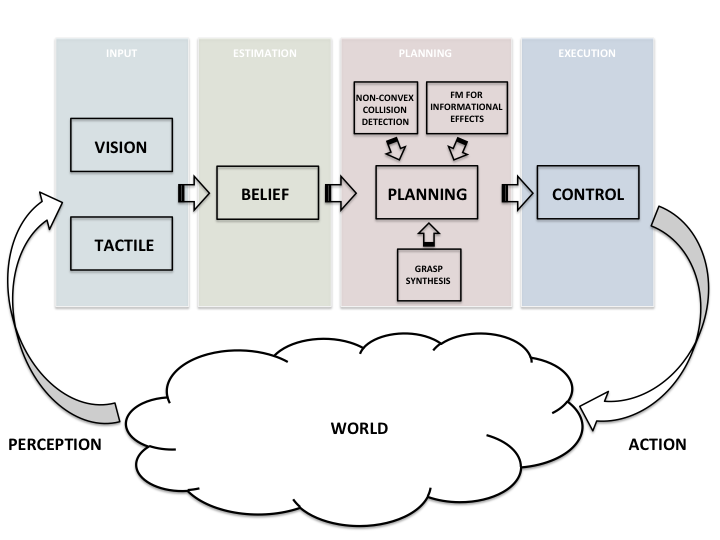
\includegraphics[width=.98\columnwidth]{../media/thesis/img/ch07_architecture.png}
}
\caption[SPAM-PLAN for grasping]{The architecture of the system is composed of 4 components: sensory input, pose estimation, motion planning and active control. The arrows show the flow of the system and its interaction with the external world. The system presented in this chapter involve 3 different modules in the motion planning phase: i) collision detection procedure for non-convex objects represented as a point cloud, ii) a forward model (FM) is used to maximise the chance of gathering tactile observations that will reduce pose uncertainty, and iii) a grasp synthesis procedure to compute grasps on point clouds. }
\label{fig:architecture}
\end{figure}

In Chap.~\ref{ch06}, the IG planner works with a cost function that allows deviations from the shortest path. These encourage gathering tactile observations that will reduce pose uncertainty in the object location. Section~\ref{sec:ch06:heuristic} showed how to reason about informational effects of an action by simply encoding the expected informational value into a cost function. Such a cost function can be minimised using any motion planning technique (here a PRM), such as the ones described in Chap~\ref{ch03}. As we have seen at the end of the previous chapter, a drawback of encoding the information value into the cost function is the extra computation during the query phase of the PRM algorithm in order to compute the likelihood of reading a contact. This requires finding the closest surface to the finger tips for each hypothesis every time a node of the PRM is in a neighbourhood of the uncertain region.
The new set of algorithms in this chapter also use the procedure described in Sec.~\ref{sec:ch07:non_convex_obj} to compute the expected (tactile) observations in the planning process (Sec.~\ref{sec:ch06:observational_model}), erasing the computational discrepancy between the two sequential re-planning algorithms. 

The rest of this chapter presents the new features implemented in the sequential re-planning algorithms in more detail.
 
%The work presented in this chapter extends the set of algorithms presented in Chap.~\ref{ch06}, such as i) integrate the method described in~\citep{bib:kopicki_2014} to compute on-the-fly target grasps, ii) efficiently plan collision-free, dexterous grasping trajectories for a non-convex object represented as point cloud, and iii) iteratively update the object pose estimate using a observational model for noisy contact sensing.  
%
%We make several assumptions. First we assume a reference model for the object is available. Nevertheless, completeness in this model is not necessary for our algorithm to work. Incomplete point clouds can be used as models. Second we assume that a separate sequence of views given by a depth camera give an incomplete point cloud which can be aligned to this model. The shape incompleteness of both model and observation of the object results in object-pose uncertainty encoded in a belief density for the pose. Given this our approach selects the optimal reach to grasp trajectory with respect to the current belief state. Second we assume that the algorithm takes as input a target grasp configuration on the object (i.e. the set of finger contacts on the model), and a pre-grasp configuration. We use the method described in~\citep{bib:kopicki_2014} to generate this target grasp for the presented object. Third we assume that the object is stationary and we actively control the compliance of the robot when in contact with the object without altering the object pose. Fourth we assume the availability of a belief state estimate of the object's pose in the form of a particle filter.
%
%The architecture of our system is shown in Fig.~\ref{fig:architecture}. Similarly to the architecture seen in Chap.~\ref{ch06}, an Asus Xtion Pro depth camera is employed to obtain a depth image. This gives an incomplete point cloud of the object surface, referred as \emph{query point cloud}. A probability density (or belief state) over the object pose is estimated as a particle set. In contrast to the previous implementation, the expected pose of the object is computed by computing the mean of the more promising cluster of particles as it will be described in Sec.~\ref{sec:ch07:state_estimator}. Using the method described in~\citep{bib:kopicki_2014} a grasp is computed for the target object, under the assumption that the object is in its expected location, and a reach-to-grasp trajectory is planned. As before, this planner works with a cost function that allows deviations from the shortest path that maximise the chance of gathering tactile observations that will reduce pose uncertainty in the object location. If unexpected observations occur during the execution of the planned trajectory, then such observations (both tactile contact and no-contact signals) collected at poses along the reach-to-grasp trajectory are used to perform a particle filter update. Re-planning then occurs with the new pose distribution, and a new reach-to-grasp trajectory can be constructed. This process is then iterated until a successful grasp is achieved.
 
%---------------------------------------------------------------------------------------------------------------------
% 	PROBLEM DOMAIN
%---------------------------------------------------------------------------------------------------------------------
%---------------------------------------------------------------------------------------------------------------------
\section{Technical contributions}\label{sec:ch07:problem_domain}

As explained, the set of algorithms presented in this chapter have a similar formulation to those in Chap.~\ref{ch06}. 
However, there are several key differences to be discussed. This section describes each of them separately.

\subsection{Mean pose estimate}\label{sec:ch07:state_estimator}

Section~\ref{sec:ch06:state_estimator} presented this as the mean of the set of particles in the belief filter. In this chapter a new state estimator is proposed. In chapter 6, the mean was estimated using a mean-shift algorithm on the particle set. This simple estimate of the mean does not work well with multi-modal beliefs. Therefore, in this chapter, I combine the mean-shift algorithm with a hierarchical clustering algorithm to compute the mean of the most promising cluster within a possible multi-modal belief.

This procedure uses the mean-shift algorithm to generate a set of cluster centres from the particle set. Each associated with: i) a score which identifies the ``goodness'' of the estimate, in terms of how well the estimate represents the entire set of particles, and ii) the number of particles that have contributed to construct the estimate. 
Let $c_i$ be the centre particle of a cluster, $C_i$, of the entire set of particles $[p_1,\dots,p_K]$. Each particle is associated with an importance sampling weight $w_k$, then the score for the cluster $C_i$ is computed as
$$
s_{C_i} = \sum_{k\in[1,\dots,K]}{w_ke^{||c_i-p_k||_Q}}
$$
where $||a||_Q$ is defined as $a^TQa$ and $Q$ is the covariance matrix of the set of particle $[p_1,\dots,p_K]$. Once a fixed number of clusters $C_i$ is generated, the procedure agglomerates the most similar clusters, if any, and computes the best estimates as the mean of the most promising cluster $C_{max}$, which is defined as:
$$
C_{max} = \arg\max_{C_i}{\frac{|C_i|}{\sum_j{|C_j|}}s_{C_i}}
$$  
where $s_{C_i}$ is the score associated with the cluster $C_i$, and $|C_i|$ is the cardinality of the cluster $C_i$ in term of number of members.

\subsection{Grasp synthesis}\label{sec:ch07:grasp_synthesis}

Section~\ref{sec:ch02:grasp_synthesis} discussed how to learn grasp types that can be generalised to novel object's shapes and discussed the work of~\citep{bib:kopicki_2014, bib:kopicki_2015}, which proposes an efficient method to learn dexterous grasp types (e.g. pinch, rim) from a single example that is able to generalise within and across object categories, and with full or partial shape information. As a minor contribution to this thesis, I have integrated this method to enable the system to generate grasps on-the-fly. A user of the system can select the grasp type which will be automatically generated on the novel object's shape.

\subsection{Re-planning}\label{sec:07:replan}

As we have seen in Chap.~\ref{ch06}, the sequential re-planning algorithm planned trajectories assuming only the maximum likelihood observations given the current belief state. Therefore we need to rely on sensory feedback during the execution of the planned trajectory in order to detect whether or not unexpected observations occur. This triggers a belief update, using the observation gathered at execution-time, and consequently a re-planning phase. 

As described in Chap.~\ref{ch06}, and in~\citep{bib:zito_workshop_iros2012, bib:zito_iros_2013}, after a contact the manipulator was moved back to a safe configuration (e.g. outside the uncertain region) prior to each new reach-to-grasp trajectory being planned. This approach was necessary for technical reasons due to the robotic platform in use. This approach was tested on DLR's Rollin Justin robot. The only way to communicate with this platform is via its own controller. This controller accepts trajectories with extra parameters to set, for example, compliance or activate/disactivate a joint's torque thresholds (or guards). However these parameters cannot be changed on-line during the execution of the trajectory and the controller forbids any movement once an active guard has been triggered. It is possible however to send a trajectory with disabled guards. Therefore the only feasible work around, after making a contact, was to withdraw the robot to a safe configuration with no active guard before the next reach to grasp attempt. This, however, is inefficient and fails to exploit the existing contact in completing the grasp.

To overcome these limitations the modified method, proposed in this chapter, has been implemented on a robotic platform called Boris. Boris' controller enables us to modify settings (compliance and thresholds) on-the-fly at execution time. This allows us to make a contact with an object, stop the robot, and then re-plan from the same configuration, while maintaining contact with the object.

In the experiments presented here, the algorithm uses torque sensors, based on current draw, at each joint of the robot's hand to detect whether or not a link of the hand is in contact with the environment. As a minor contribution to this thesis, a contact detection module has been developed to remove the noise from the sensors, which we will discuss briefly now.

\subsection{Detecting contacts}\label{sec:07:detecting_contacts}

As mentioned, the system developed in this thesis relies on the torque sensors based on the current draw at each joint of the DLR Hit Hand II. Figure~\ref{fig:07:torques} shows the torque signal received from the robot hand during a reach-to-grasp trajectory. Joint 0 (blue) is responsible for the abduction movement, while Joint 1 (green) and 2 (red) are responsible for flexion movements. The fourth joint (Joint 3) of the DLR HIT Hand II is mechanically coupled with Joint 2, so it is not shown in the figure. 

When the robot is commanded to move, the inertias of each finger link, cause significant torque signals to be sensed, even without any contact with external objects. Therefore, an important practical problem is how to remove that portion of the torque signal that is due to the robot's own motion, in order to detect torque changes due to external contacts. To do so, a Gaussian low-pass filter with a fixed window size is used to filter out the noise. Alg.~\ref{alg:lowpass_filter} shows the pseudo code for a low-pass filter. The functions diff($\cdot$), normpdf($\cdot$) and conv($\cdot$) are considered as in the MATLAB API, where diff($X$) calculates differences between adjacent elements of $X$ along the first array dimension whose size does not equal 1; normpdf($X,\mu,\sigma$) computes the pdf at each of the values in $X$ using the normal distribution with mean $\mu$ and standard deviation $\sigma$; and conv($u,v$) returns the convolution of vectors $u$ and $v$. In this implementation $mask\_size=2$ and $\sigma=1.0$, while $data$ is the vector of torques for a particular joint. The length of $data$ is equal to the selected window size. In this implementation the window size is equal to 40, which means $data$ contains the latest 40 readings from the joint's torque.  

\begin{algorithm} [t!]                   
\caption{LOWPASS\_FILTER}          
\label{alg:lowpass_filter}                           
\begin{algorithmic}                    
\REQUIRE data, mask\_size, $\sigma$
\ENSURE L
\STATE x $\gets$ [-mask\_size:.1:mask\_size]
\STATE mask $\gets$ diff(normpdf(x,0,$\sigma$))
\STATE L $\gets$ conv(data, mask)
\end{algorithmic}
\end{algorithm}

Figure~\ref{fig:07:filtered_torques} shows the corresponding filtered signals along the trajectory. Ideally, we would like to have a zero signal until the finger makes a contact. However, this is not possible to achieve due to the activity of the joints' actuators, the acceleration of the hand along the trajectory and the changes in the gravity vector according to the changes in the orientation of the hand. Nevertheless, the system allows us to define thresholds to further filter the signals. Via empirical experiments on Boris we determined that a threshold of 0.05 gives an appropriate trade-off between false positives and false negatives.

\begin{figure}[!t]
\centering
 \begin{subfigure}[t]{0.98\textwidth}
       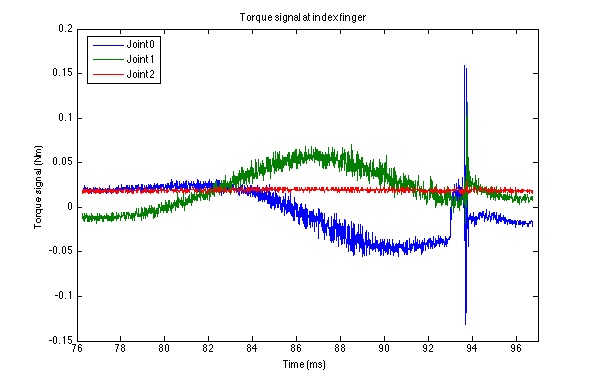
\includegraphics[height=7.5cm,width=15cm]{../media/thesis/img/torque_index.png}
       \caption{}\label{fig:07:torques}
  \end{subfigure} 
 \vspace{2mm}
  \begin{subfigure}[t]{0.98\textwidth}
     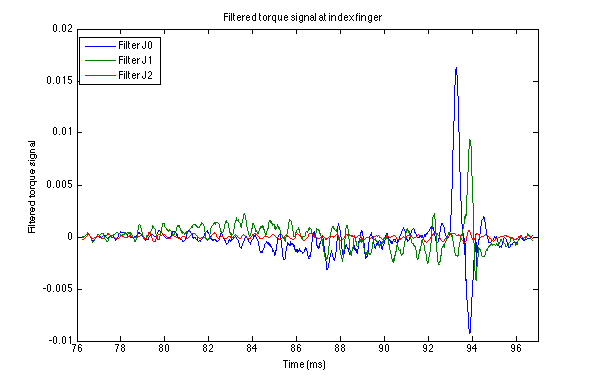
\includegraphics[height=7.5cm,width=15cm]{../media/thesis/img/filtered_torque_index.png}
     \caption{}\label{fig:07:filtered_torques}
  \end{subfigure}
\caption[Filtered torque signals]{The images show the real torque signals~\subref{fig:07:torques} and the corresponding Gaussian low-pass filter signal~\subref{fig:07:filtered_torques} for each joint of the index finger of the DLR Hit Hand II during a reach-to-grasp trajectory. Joint 0 (blue) is responsible for the abduction movement, while Joint 1 (green) and 2 (red) are responsible for flexion movement. The fourth joint (Joint 3) of the DLR Hit Hand II is coupled with Joint 2, so it is not shown. The torque signal is plotted over time. At approximately 93ms a contact with the target object is made, as shown by the increasing of the torque signals.}
\label{fig:07:torque_signal}
\end{figure}

\subsection{Planning a dexterous grasping trajectory for non-convex objects}\label{sec:ch07:non_convex_obj}
% TODO:
% collision only with the estimated pose.
% if the model is poor than the collision detection is unreliable.

The implementation of this planner uses a modified version of Probabilistic Roadmap (PRM) planning,~\citep{bib:kavraki_1996}, to plan trajectories. Crucially, sampling-based approaches like PRMs rely on the ability of rejecting points that are in collision. Testing collision between simple geometrical primitives, such as planes, spheres or cubes, is substantially faster than between non-convex polyhedra. On the other hand, if an object to be grasped is wrapped in a simple primitive bounding box, to achieve computational efficiency, many grasps would simply be impossible to achieve. The left image in Fig~\ref{fig:07:grasps} shows the case of a grasp over the rim of a jug. This grasp requires the thumb to penetrate inside the convex hull of the object. Thus, even if this configuration does not produce any true collisions, it would be rejected by such ``naive'' collision detection. 

\begin{figure}[!t]
\centering
 \begin{subfigure}[t]{0.48\textwidth}
       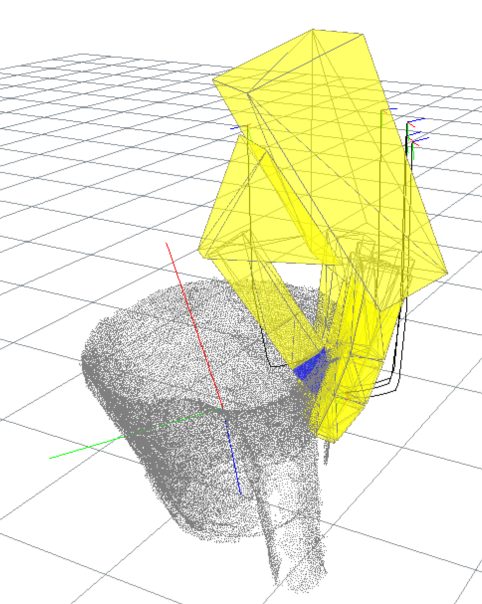
\includegraphics[width=.98\columnwidth]{../media/thesis/img/jug.png}
       \caption{}\label{fig:07:jug_rim}
  \end{subfigure} 
  \quad
   \begin{subfigure}[t]{0.48\textwidth}
       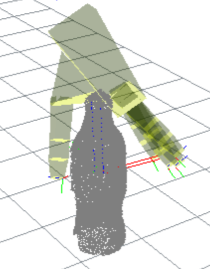
\includegraphics[width=.98\columnwidth]{../media/thesis/img/coke.png}
       \caption{}\label{fig:07:coke_top}
  \end{subfigure} 
  \vspace{2mm}
  \begin{subfigure}[t]{0.48\textwidth}
       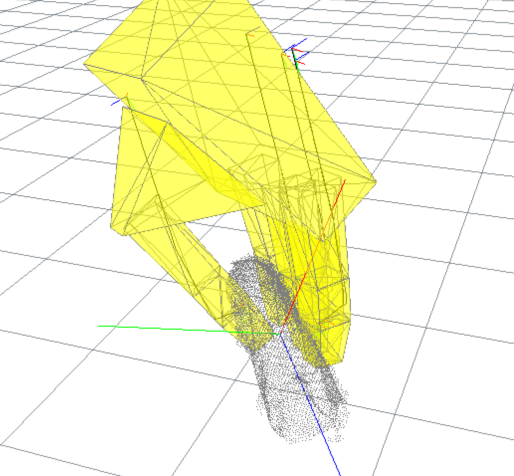
\includegraphics[width=.98\columnwidth]{../media/thesis/img/stapler_rim.png}
       \caption{}\label{fig:07:stapler_rim}
  \end{subfigure} 
  \quad
   \begin{subfigure}[t]{0.48\textwidth}
       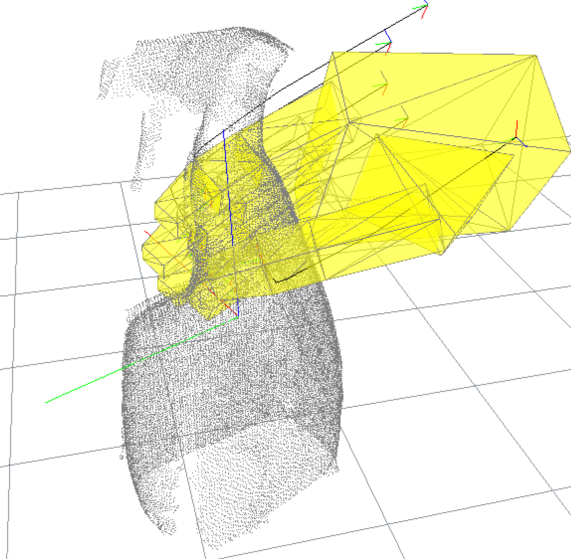
\includegraphics[width=.98\columnwidth]{../media/thesis/img/mrmuscle_rim.png}
       \caption{}\label{fig:07:mrmuscle_rim}
  \end{subfigure} 
\caption[Object models with associated grasp]{Models of the objects and their associated grasps. The image~\subref{fig:07:jug_rim} shows a rim grasp on a jug. In this case, the target grasp requires that the thumb be placed on the internal surface of the object, thereby penetrating inside the convex hull. The image~\subref{fig:07:coke_rim} shows a top grasp on a bottle of coke. The images~\subref{fig:07:stapler_rim} and~\subref{fig:07:mrmuscle_rim} show respectively a rim grasp on a stapler and a Mr Muscle spray bottle. The grasp configurations are computed using the method described in~\citep{bib:kopicki_2014}.}
\label{fig:07:grasps}
\end{figure}

Here a fast and efficient collision detection module to cope with objects represented by a point cloud is proposed. Whilst the robot's rigid links are represented by an open-chain of convex polyhedra, the object to be grasped is represented by a 2-level structure. The first level of this structure wraps the point cloud in a bounding box. This level can efficiently avoid checking collisions between the robot's links and the object to be grasped when they are far apart. The second level contains the point cloud organised in a KD-Tree. The KD-Tree implementation is based on the FLANN library~\citep{bib:muja_2014}. An example of the 2-level collision detection is shown in Fig.~\ref{fig:bounding_box}.

\begin{figure}[!t]
\centerline{
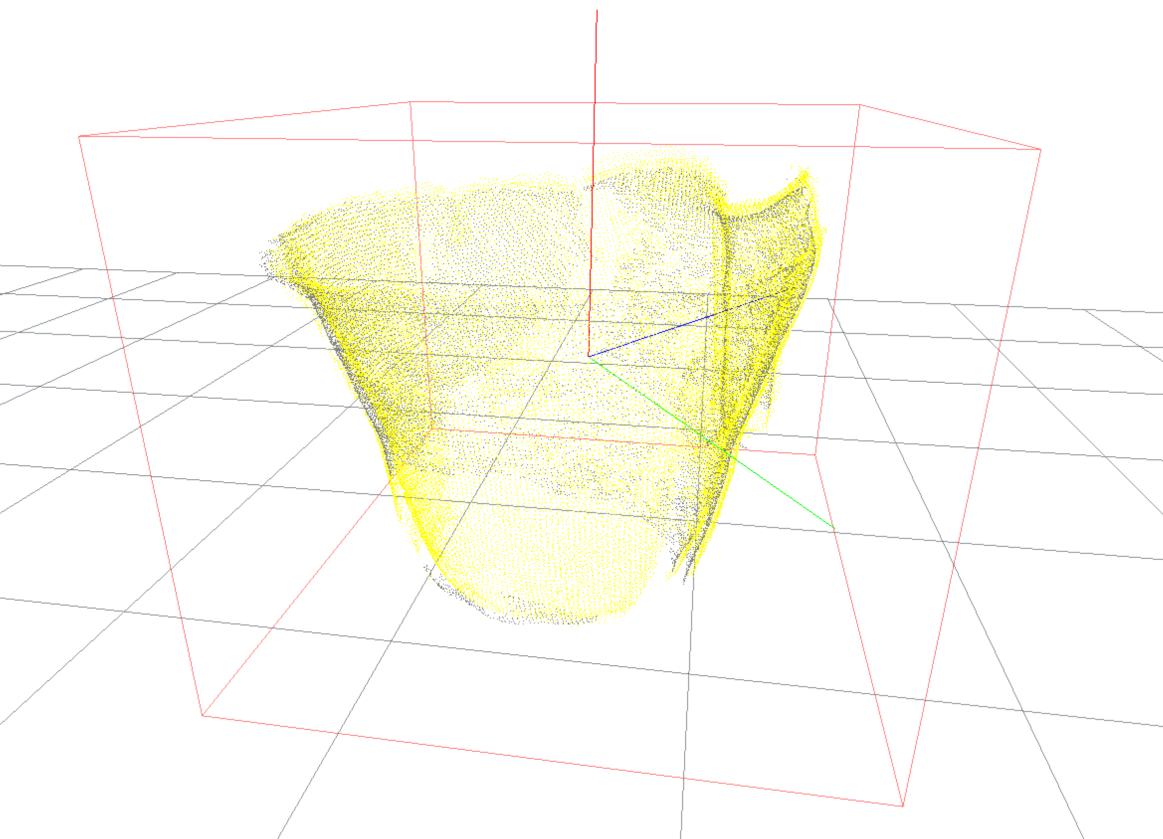
\includegraphics[width=.48\columnwidth]{../media/thesis/img/bounding_box.png}
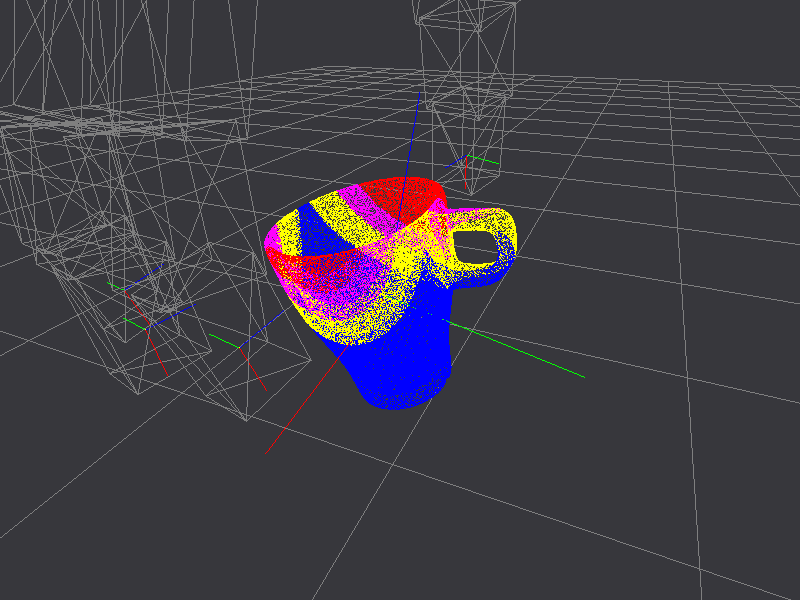
\includegraphics[width=.48\columnwidth]{../media/thesis/img/contacts.png}
}
\caption[Hierarchical collision detection]{The left image shows the target object to be grasped. In this case the object is a jug. The grey point cloud represents the ground truth pose of the object, as it was acquired by a noiseless input source. The yellow point cloud identifies the best pose estimate. The yellow point cloud is organised as a KD-Tree for faster collision detections. The red box represents the bounding box, which prevents unnecessary collision checking between the object and robot's links when they are far apart. The right image shows a point cloud for a mug and the robot hand's configuration. Each point is coloured with respect to the relative distance to the closest finger's link of the robot's hand: red (closest) to blue (furthest). }
\label{fig:bounding_box}
\end{figure}

%We assume that the collision with the object to be grasp can only happen with the bodies of the robotic hand. Thus 
The planning process uses a collision detection in two cases: i) to reject PRM nodes in collision with an object and ii) to compute the information value for each edge of the PRM. In the former case, the planning process only targets the object as if it were in its expected location (the mean pose of the density function), therefore only the mean pose is used for collision detection. In contrast, the latter case requires us to compute the information value for all the sub-sampled hypotheses. In both cases, when at least one bounding box of the robot collides with the bounding box of the object, the second level of the collision detection module is called. By querying the KD-Tree it is possible to retrieve the closest points on the surface of the object to the robot's links, see Fig.~\ref{fig:bounding_box} (right). Each point is then checked to determine whether it collides or not, or to estimate the likelihood of observing a contact.  

Algorithm~\ref{alg:get_penetration} shows the core of the proposed collision detection procedure. This procedure computes a \emph{penetration} value for a particular point $p$ in the point cloud and a set of bounds for the robot hand. The penetration value is an approximation of the distance between $p$ and the closest surface of the robot hand, and it is positive if the point sits inside the bounds, or negative otherwise. Algorithm~\ref{alg:check_collision} shows the collision detection procedure used to reject a robot pose in collision. In this case, the procedure rejects a robot pose if the associated penetration value is greater than or equal to zero. It is also possible to treat a point $p$ as a sphere with centre $p$ and radius $\rho$ and this allows us to plan more conservative trajectories. 

Let $b_i$ be the boundary of the $i-$th link in the robot hand, represented as a convex polyhedron. Figure~\ref{fig:surface_distance} shows the boundary $b_i$ as a simple 6 faced polyhedron. Then $b_i$ is composed of a set of triangles $T_i=[t_1,\dots,t_M]$ and a reference frame $O_i\in SE(3)$. Each triangle $t_j\in T_i$ is composed of three vertices $v_{j1},v_{j2},v_{j3}$ and it is possible to compute the normalised normal vector $n_j$ as
$$
n=(v_2-v_1)(v_3-v_1)
$$
$$
n_j=\frac{n}{||n||}
$$
Note that either $n_j$ or $-n_j$ would be a normal for the triangle $t_j$. The procedure chooses $n_j$ with the direction that points outside the polyhedron, as shown in Fig.~\ref{fig:surface_distance}. 
Note that since all the normals are computed to point outside the boundary, for a point $p$ to be in collision it must satisfy the following condition:
$$
||v_{j1}||_{O_i}-n_j^Tp > 0, \qquad\forall j\in[1,\dots,M]
$$
where $||v_{j1}||_{O_i}$ is the distance of the triangle $t_j$ from the reference frame $O_i$, approximated as the distance to its first vertex $v_j1$, and $n_j^Tp$ is the dot product between the normalised normal $n_j$ and the point $p$. In classical geometry, the distance between a triangle and a point is computed as the length of the projection of the point $p$ onto the triangle or, if the projection does not sit on the triangle's surface, distance to the point's projection onto the closest edge of the triangle. In order to speed up the computation, the implementation I propose computes for each triangle the penetration value as the distance between the point $p$ and the first vertex, $v_1$, of the closest triangle. If the point sits outside the boundary $b_j$, the penetration value is the negative of the computed distance. If the triangles $t_j$ are small, this is a good approximation.

\begin{figure}[!t]
\centerline{
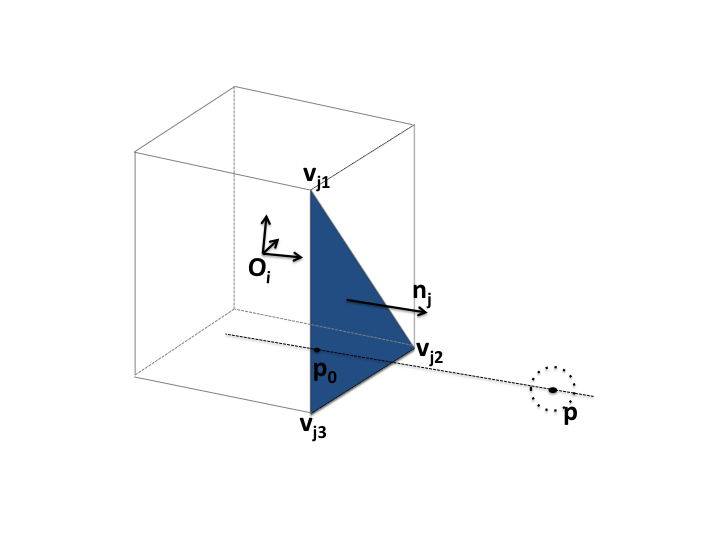
\includegraphics[width=.88\columnwidth]{../media/thesis/img/surface_distance.png}
}
\caption[Distance from a mesh triangle and a point]{The image shows a mesh triangle, $t_j$, of vertices $v_{j1},v_{j2}, v_{j3}$ and the normalised normal vector $n_j$, the reference frame of the mesh $O_j$ and the point $p$ with its projection on the triangle surface. The projection is the point $p_0$ on the triangle surface which intersects the line passing through the point $p$ with the same direction of $n_j$. The dotted line around the point $p$ represents the spherical bounding box used for planning more conservative trajectories.}
\label{fig:surface_distance}
\end{figure}

\begin{algorithm} [t!]                   
\caption{CHECK\_COLLISION}          
\label{alg:check_collision}                           
\begin{algorithmic}                    
\REQUIRE robot\_pose, hand\_bounds, kdtree, neighbours, $\rho$
\STATE closest\_points $\gets$ KNN\_SEARCH(kdtree, robot\_pose, neighbours)
\FORALL{$b_i\in$  hand\_bounds}
	\STATE $d \gets$ GET\_PENETRATION($b_i$, closest\_points)
	\IF{$d> -\rho$}
		\RETURN true 
	\ENDIF
\ENDFOR
\RETURN false
\end{algorithmic}
\end{algorithm}

\begin{algorithm} [t!]                   
\caption{GET\_PENETRATION}          
\label{alg:get_penetration}                           
\begin{algorithmic}                    
\REQUIRE $b_i$, closest\_points
\STATE distance $\gets +\infty$
\FORALL{ $p\in$ closest\_points}
	\STATE $d \gets$ GET\_PENETRATION\_PER\_BOUND($b_i,p$)
	\IF{distance $> d$}
		\STATE distance $\gets d$
	\ENDIF
\ENDFOR
\RETURN distance
\end{algorithmic}
\end{algorithm}

\begin{algorithm} [t!]                   
\caption{GET\_PENETRATION\_PER\_BOUND}          
\label{alg:get_penetration2}                           
\begin{algorithmic}                    
\REQUIRE $b_i,p$
\STATE distance $\gets +\infty$
\STATE direction $\gets +1$ 
\FORALL{$t_j\in b_i$}
	\STATE $d_1 \gets ||tj.v_{j1}-p||$
	\IF{distance $> d_1$}
		\STATE distance $\gets d_1$
	\ENDIF
	\IF{direction $> 0$}
		\STATE $d_2 \gets ||t_j.v_{j1}||_{O_i} - t_j.n_j^Tp$
		\IF{$d_2 < 0$}
			\STATE direction $\gets -1$
		\ENDIF
	\ENDIF 
\ENDFOR
\RETURN direction$\cdot$distance
\end{algorithmic}
\end{algorithm}

Note that the lack of complete information about the object's shape may affect collision detection, leading to a reach-to-grasp trajectory which passes through the object. In a real scenario, however the tactile observation that will be generated will cause the robot to stop and the current belief state to update. One limitation of the current implementation, is that this approach does not reason about the relative likelihood that the unexpected observation is given by a mis-estimation of the object pose versus lack of shape information; it simply updates the belief density over the object-pose. As future work,  the aim would be to treat this problem as a SLAM problem, which will enable us to compensate for initially incomplete shape information in the object model. 


\subsection{Terminal conditions}

The sequential re-planning algorithm terminates its execution when no unexpected contacts occur and the target grasp is achieved. Since we do not have mesh models of the object to be grasped we cannot rely on grasp quality measures (discussed in Sec.~\ref{sec:ch02:grasp_stability}) to signal successful termination of the algorithm. Nonetheless, in simulation it is possible to measure the displacement error between the grasp configuration for the final object-pose estimate and the ground truth. A user-defined threshold of tolerance is used to identify whether the grasp has succeeded. On the real robot, the success of the grasp is evaluated by lifting the object. If the robot can hold the object, the grasp is considered successful.


%\subsection{Observation model}\label{sec:ch07:observational_model}
%
%As discussed in Sec.~\ref{sec:ch06:observational_model}, a robotic manipulator is composed of chains and joints linked together. The ordered set $\mathbf{M}$ identifies the ``fingers'' of the robotic hand. 
%
%
%Mathematically we formalise the likelihood of observing a contact for each finger of the robot as an exponential distribution over the Euclidean distance, $d_{ji}$, between the finger tip's pose, $W(x(j))$, and the closest surface of the object assumed to be in pose $p^i$. Note that, for this work, we limited our observation model to contacts which may occur on the internal surface of fingers. This directly affects our planner which rewards trajectories that would generate contacts on the finger tips rather than on the back side of the fingers. Therefore for any $j\in\bar{M}$ we write
%$$
%p(y(j)=1|x(j), p^i)=
%\begin{cases}
%  \eta\exp(-\lambda d_{ji}) & \text{if }d_{ji}\leq d_{max} \\
%	& \text{and }\langle n_{xj},\hat{n_{p^i}}\rangle < 0 \\
%  0 & \text{otherwise}
%\end{cases}
%%p(y_{t}|x_{t}, p^{i})=\prod_{j\in\hat{M}}{p(y_{y}(j)|x_{t}(j),p^{i})}
%$$
%where $\langle n_{xj},\hat{n}_{p^i}\rangle$ is the inner product of, respectively, the $j^{th}$ finger tip's normal and the estimated object surface's normal, and $d_{max}$ describes a maximum range in which the likelihood of reading a contact is not zero, and $\eta$ is a normaliser. This allows us to rewrite the likelihood of reading a contact on the force/torque sensors of the robot, $h(x,p^i),i\in[1,k]$ with $j_1,\ldots,j_m\in\bar{M}$ as follows,
%$$
%\begin{aligned}
%h(x,p^i)=[p(y(j_1)=1|x(j_1),p^i),\dots,p(y(j_n)=1|x(j_m),p^i)]^T
%\end{aligned}
%$$
%
%
% 
%
%
%\subsection{Belief update}
%
%Once a trajectory is executed and a real (unexpected) observation $y$ is detected, we update our belief state according to Bayes' rule. We represent our belief state as a set of $N$ particles $b_t=\{b_t^z\}_{z=1}^{N}$. In a particle filter fashion we update the weight of each particle $b_t^z$, $z\in\{1,\ldots,N\}$, as follows
%$$
%p(y|x, b_t^z)=\prod_{j\in\hat{M}}{p(y_{t}(j)|x_{t}(j),b_t^z)}
%$$
%and then we execute a resampling step which generates a posterior distribution $b_{t+1}$ as new set of particles $\{b_{t+1}^z\}_{z=1}^{N}$.
%
%In simulation we assume that there are no false dectections. However it is possible to distinguish whether or not a contact occurs between the object to be grasped and the robot's end-effector. For example, in case a contact with the environment is detected we skip the belief update step and we move the robot back to a safe configuration before triggering the re-planning.
%
%---------------------------------------------------------------------------------------------------------------------
% 	EXPERIMENTS
%---------------------------------------------------------------------------------------------------------------------
%---------------------------------------------------------------------------------------------------------------------

\section{Results}\label{sec:ch07:results}

This section presents the experimental results used to evaluate the new set of algorithms presented in this chapter. As in Chap.~\ref{ch06}, three strategies for planning dexterous reach-to-grasp trajectories are evaluated in both the real robot platform Boris and a simulated environment:
\begin{itemize}
\item ELEMENTARY: an open-loop trajectory towards the expected object pose without re-planning.
\item MYCROFT: a sequential re-planning algorithm without information gathering. 
\item IR3NE: a sequential re-planning algorithm with information gathering. 
\end{itemize}

In this evaluation the aim is to show that sequential re-planning is capable of achieving higher grasp success rates than single grasp attempts in presence of non-Gaussian object-pose uncertainty in 6 dimensions. It also shows, as in the previous chapter, that planning trajectories that maximise information gain result in fewer re-planning iterations to achieve a grasp. 

First, Sec.~\ref{sec:07:boris_results} presents empirical results collected on 20 trials for a single object (a jug) using a real robot, in which the ability of these three different strategies to achieve a grasp configuration is tested as well as the benefits of using a mean-shift algorithm with hierarchical clustering to compute the estimate of the object's pose. 

In addition, Sec.~\ref{sec:07:simulated_results} presents the results collected on 120 trials in simulation for four objects: a jug, a bottle of coke, a stapler and a Mr Muscle spray bottle. In these experiments, a mean-shift algorithm is still used to compute the pose estimate, and the aim is to evaluate the ability of the three strategies to achieve a grasp configuration. 

\subsection{Experiments on the robot Boris}\label{sec:07:boris_results}

These experiments are composed of 2 runs of 20 trials each (10 trials using MYCROFT and 10 using IR3NE). The results for the ELEMENTARY strategy are extrapolated from the results collected for MYCROFT, in the sense that the two approaches construct a reach-to-grasp trajectory minimising the same cost function, therefore if MYCROFT achieves (or fails to achieve) a grasp at the first iteration, the ELEMENTARY also would have succeeded (failed) as well. 
 
For both set of trials only one object has been used: the jug shown in Fig.~\ref{fig:bounding_box}. A dense point cloud, representing the object model, is assumed to be available at the beginning of each run. This object model is acquired by scanning the operational workspace (Sec.~\ref{sec:ch03:operational_ws}) with a depth camera from 6 different views. These views are merged to generate a single point cloud of the object model. This pre-processing aligns the single view point clouds, registering and eliminating outlier points.

At each trial, the target object is placed on a table in front of the robot, within the robot's operational workspace, in a different configuration. In this case, the query point cloud is acquired by scanning the operational workspace from only 3 different views. Once these views are aligned and registered, Boris estimates the belief state with a set of particles. The first run used a mean-shift algorithm combined with the hierarchical clustering algorithm, as presented in Sec.~\ref{sec:ch07:state_estimator}, to estimate the object's mean pose. The second run used only the single mean-shift algorithm as described in Sec.~\ref{sec:ch06:state_estimator}.

\begin{figure}[!t]
\centerline{
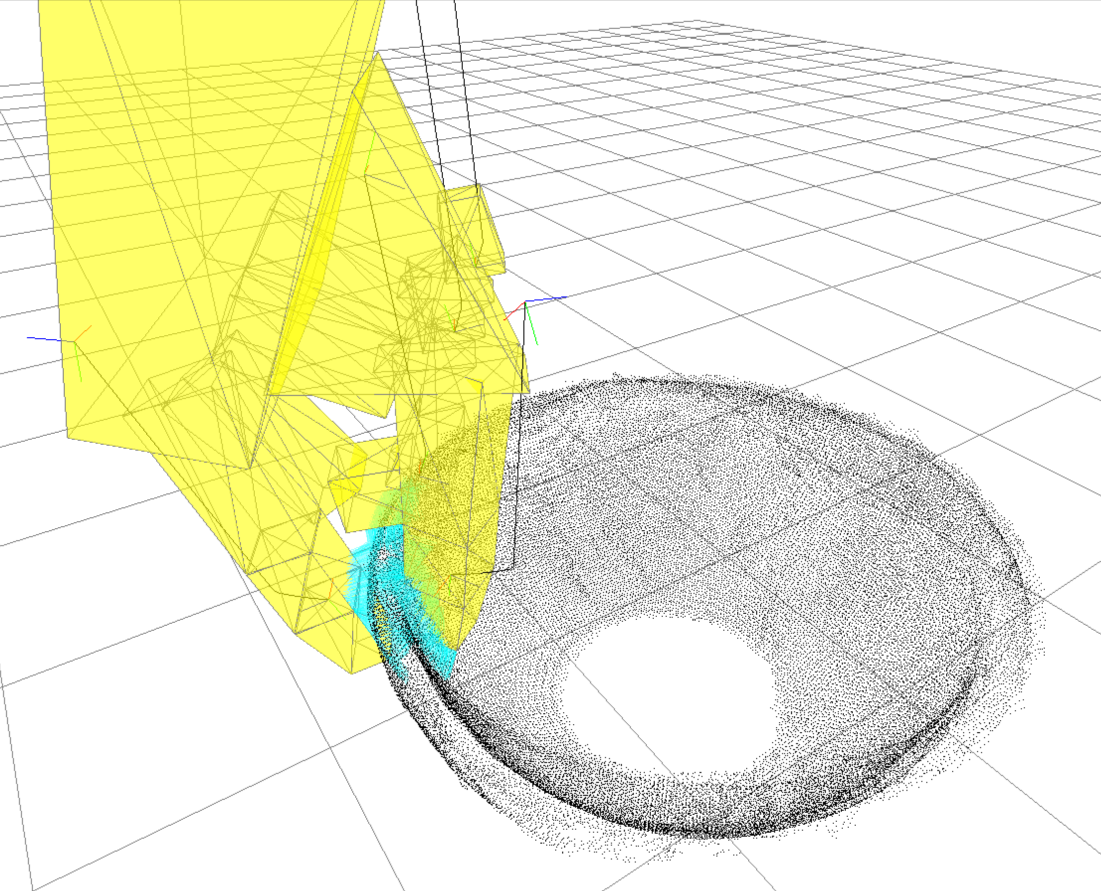
\includegraphics[width=.48\columnwidth]{../media/thesis/img/bowllarge_pinchsupp.png}
\qquad
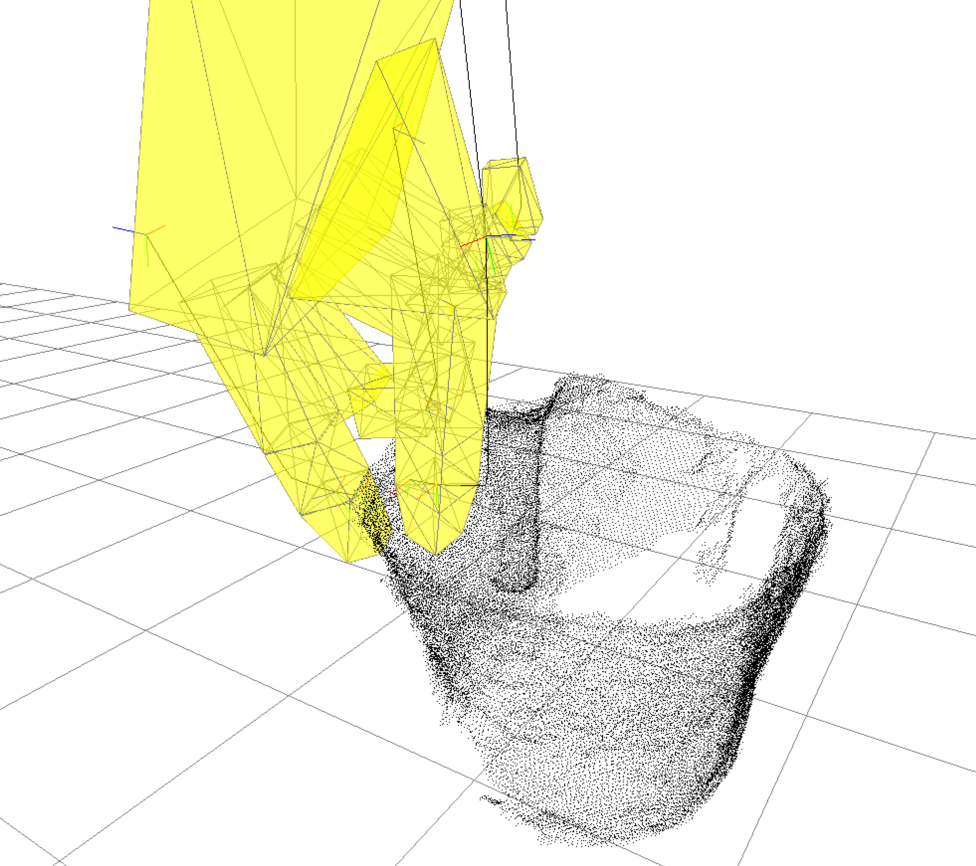
\includegraphics[width=.48\columnwidth]{../media/thesis/img/jug_pinchsupp.png}
}
\caption[Pinch with support grasp]{Pinch with support grasp learned on a bowl and transferred to a jug, using the method described in~\citep{bib:kopicki_2014}. The image on the left shows the learned contact model (blue points) for all the fingers involved in the grasp. The right image shows a possible grasp adaptation on a jug.}
\label{fig:07:bowllarge_pinchsupp}
\end{figure}

In both runs, a target grasp for the jug is computed by adapting a pinch with support grasp learned on a bowl. The training and test grasps are shown in Fig.~\ref{fig:07:bowllarge_pinchsupp}. Then a reach-to-grasp trajectory is computed and performed. A trial is considered successful if Boris can converge to the target grasp configuration and lift the object from the table surface. 

Figure~\ref{fig:07:jug_boris_results} summarises the empirical results collected. In order to test the ability of a sequential re-planning algorithm to converge to the ``true'' pose of the object, a ground truth pose of the object is calculated at the beginning of each trial by using the same model-fitting algorithm as used in Sec.~\ref{sec:ch06:state_estimator}, but sampling 500 times more features. The algorithms have no knowledge of the ground truth pose.

The results are organised in Fig.~\ref{fig:07:jug_boris_results} as follows:
\begin{itemize}
\item The number of average planning iterations across all the trials for each run, for both the re-planning strategies: MYCROFT and IR3NE (Fig.~\ref{fig:07:jug_boris_results} top left chart). 

\item The success rate across all the trials for each run, in the sense of their ability to converge to the planned grasp for all the three strategies (Fig.~\ref{fig:07:jug_boris_results} top right chart). 

\item The averaged reduction in the positional error between the estimated location and the ground truth across all the trials for each run. The error is computed as the Euclidean distance in a 3D space for both strategies: MYCROFT (middle left chart) and IR3NE (Fig.~\ref{fig:07:jug_boris_results} middle right chart).

\item The averaged reduction in the rotational error between the estimated rotation and the ground truth across all the trials for each run. The error is computed as the distance in the quaternion space for both strategies: MYCROFT (bottom left chart) and IR3NE (Fig.~\ref{fig:07:jug_boris_results} bottom right chart). The rotational error is computed for each orientation on the unit hypersphere in 4D quaternion space, and then measure displacement as the length of the arc of the geodesic which connects these two points.
\end{itemize}

Section~\ref{sec:07:boris_discussion} discusses the presented results. 

\begin{figure}[!ht]
\centerline{
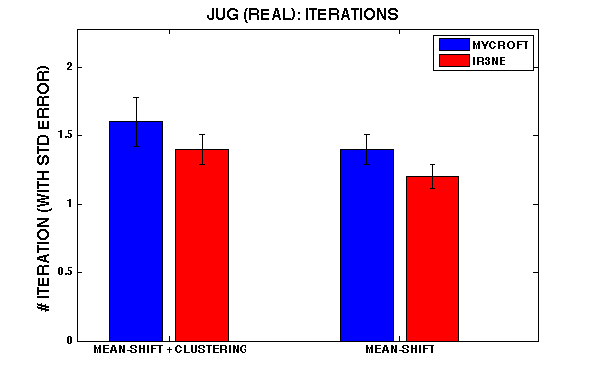
\includegraphics[width=.47\columnwidth]{../media/thesis/img/jug_boris_iterations.png}
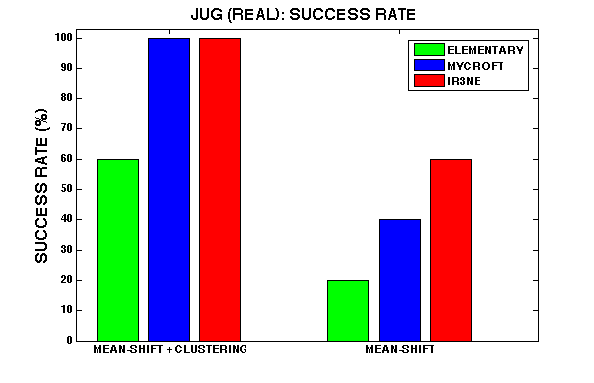
\includegraphics[width=.47\columnwidth]{../media/thesis/img/jug_boris_success_rate.png}
}
\centerline{
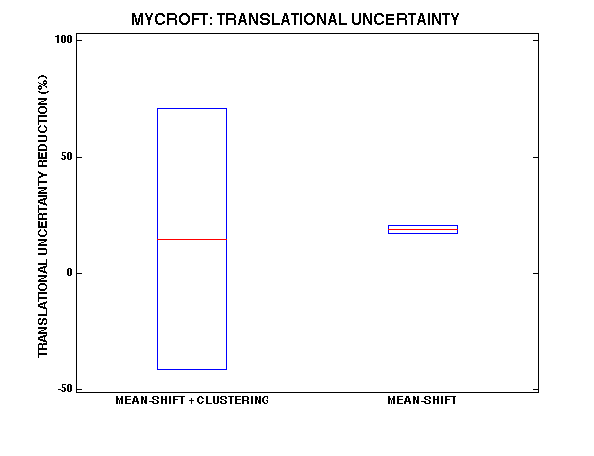
\includegraphics[width=.47\columnwidth]{../media/thesis/img/jug_boris_mycroft_lin_unc.png}
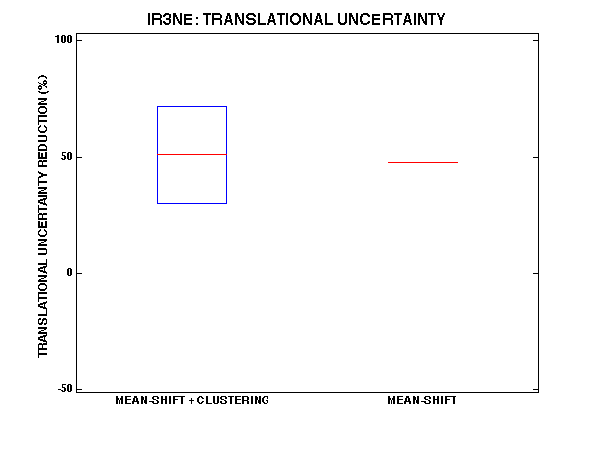
\includegraphics[width=.47\columnwidth]{../media/thesis/img/jug_boris_irene_lin_unc.png}
}
\centerline{
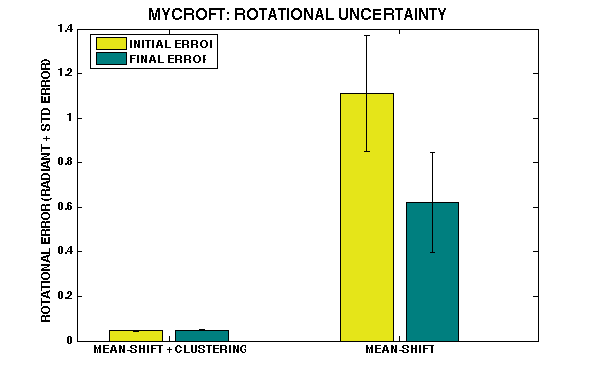
\includegraphics[width=.47\columnwidth]{../media/thesis/img/jug_boris_mycroft_rot_unc.png}
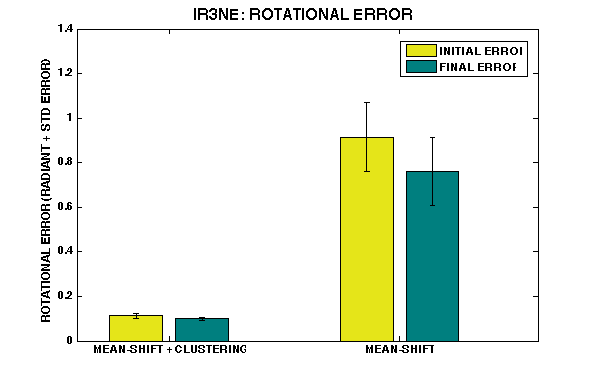
\includegraphics[width=.47\columnwidth]{../media/thesis/img/jug_boris_irene_rot_unc.png}
}

\caption[Empirical results on Boris]{Empirical results on the Boris robot platform. The results refer to 2 sets of 10 trials on a jug. Three strategies were used: ELEMENTARY (green), MYCROFT (blue), IR3NE (red). Two conditions are presented. The first uses a mean-shift algorithm combined with a hierarchical clustering algorithm to estimate the object's pose. The second uses only a mean-shift algorithm. The top left chart presents the averaged number of iterations across the trials to reach a grasp. The top right chart shows the success rates across the trials. The middle row shows how the initial linear uncertainty (in percentile) is reduced by sequential re-planning until the algorithms converge to a grasp. The bottom row presents the reduction in the rotational uncertainty. Yellow bars represent the initial rotational error, while green bars are the final error. The rotational error is computed in quaternions where similar rotations yield to error value close to zero and rotations with 180 degrees difference yield an error value of 1.}
\label{fig:07:jug_boris_results}
\end{figure}


\subsection{Experiments in a virtual environment}\label{sec:07:simulated_results}

The experiments are composed of 120 trials per object in a virtual environment: a jug, a coke bottle, a stapler and a Mr Muscle spray bottle. Each trial has a different initial probability density over the object pose. We tested the ability of different strategies to achieve a grasp configuration. The algorithm has a model of the object to be grasped, in the form of a dense point cloud, computed by scanning the object with a depth camera from 7 different views. As before, these views are pre-processed to generate a single point cloud of the object model. The pre-processing aligns the single view point clouds, registering and eliminating outlier points. Figure~\ref{fig:07:grasps} shows the pre-processed point clouds of each simulated object, and the associated target grasp configurations. For these experiments, the models are composed of 7 single-view point clouds, apart from the bottle of coke which is composed of only 5 views. 

The algorithms have been tested under the hypothesis that, at each trial, the object is displaced to a different position - but still in the dexterous workspace of the robot - and the robot has to attempt a grasp even if the new point cloud is not as dense as the model point cloud. In simulation, we achieve this by applying a rigid body transformation to the single-view point cloud to move it to a different location within the dexterous workspace of the manipulator. Four different conditions have been tested. In each condition we randomly selected either 1, 3, 5 or 7 view point clouds from the 7 single-views collected, in order to simulate real situations in which the robot's depth camera has been able to observe smaller or larger parts of the object. Once the subset of views has been selected and moved to the simulated object location, the state estimation procedure described in~\ref{sec:ch06:state_estimator} is performed.   

Figures~\ref{fig:07:jug_results},~\ref{fig:07:coke_results},~\ref{fig:07:stapler_results}, and~\ref{fig:07:mrmuscle_results} summarise the data collected in our experiments. For each condition mention above, a model coverage is computed, in terms of which percentage of the model surface was covered by the merged point clouds from the individual views. All the results are compared with respect to the model coverage in percentage terms. Again, a ``ground truth'' pose for the object is calculated at the beginning of each trial by using the same model-fitting algorithm used in Sec.~\ref{sec:ch06:state_estimator}, but sampling 500 times more features. The algorithms have no knowledge of the ground truth pose, however in the virtual environment the ground truth is used to model the real object location, and is used to trigger simulated contacts with the robot hand. These simulated contacts cause the sequential re-planning algorithm to stop and update the belief state.   

The results in Figures~\ref{fig:07:jug_results},~\ref{fig:07:coke_results},~\ref{fig:07:stapler_results}, and~\ref{fig:07:mrmuscle_results} are organised similarly to the experiments on the real robot:
\begin{itemize}
\item The number of average planning iterations across all the trials for each condition (1, 3, 5, and 7 single-view query), for both the re-planning strategies: MYCROFT and IR3NE (top left chart). 

\item The success rate across all the trials for each condition, in the sense of their ability to converge to a grasp for all the three strategies (top right chart). 

\item The average reduction in the positional error between the estimated location and the ground truth across all the trials for each condition. The error is computed as the Euclidean distance in a 3D space for both strategies: MYCROFT (middle left chart) and IR3NE (middle right chart).

\item The average reduction in the rotational error between the estimated rotation and the ground truth across all the trials for each condition. The error is computed as the distance in the quaternion space for both strategies: MYCROFT (bottom left chart) and IR3NE (bottom right chart). The rotational error is computed for each orientation on the unit hypersphere in 4D quaternion space, and then measure displacement as the length of the arc of the geodesic which connects these two points.
\end{itemize}

Section~\ref{sec:07:simulated_results_discussion} discusses the presented results and illustrates the behaviour of the sequential re-planning approach (IR3NE) generated by one simulated trial.

\begin{figure}[!ht]
\centerline{
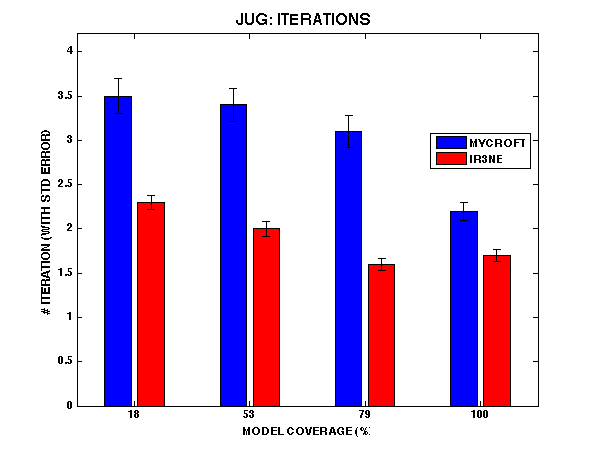
\includegraphics[width=.47\columnwidth]{../media/thesis/img/jug_iterations.png}
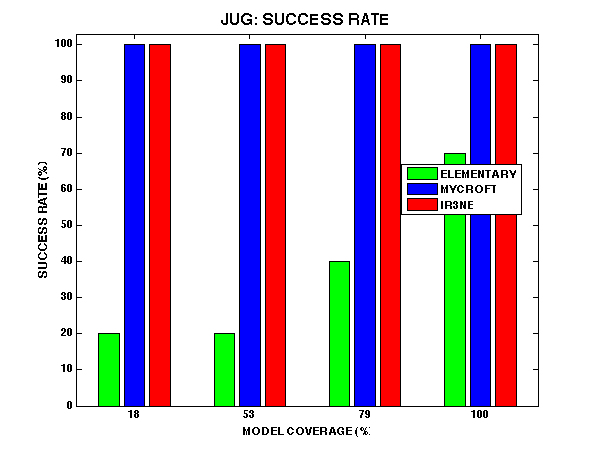
\includegraphics[width=.47\columnwidth]{../media/thesis/img/jug_success_rate.png}
}
\centerline{
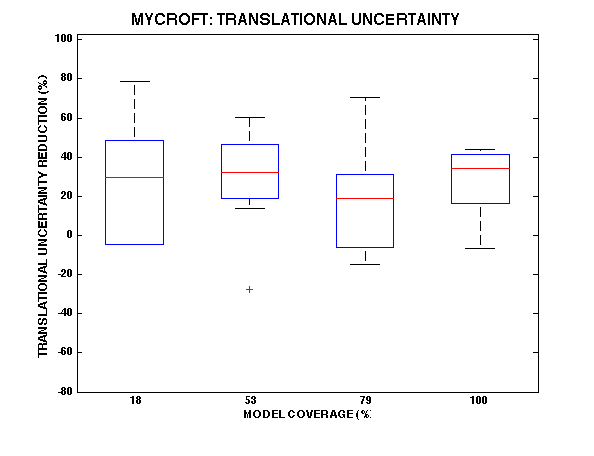
\includegraphics[width=.47\columnwidth]{../media/thesis/img/jug_mycroft_lin_unc.png}
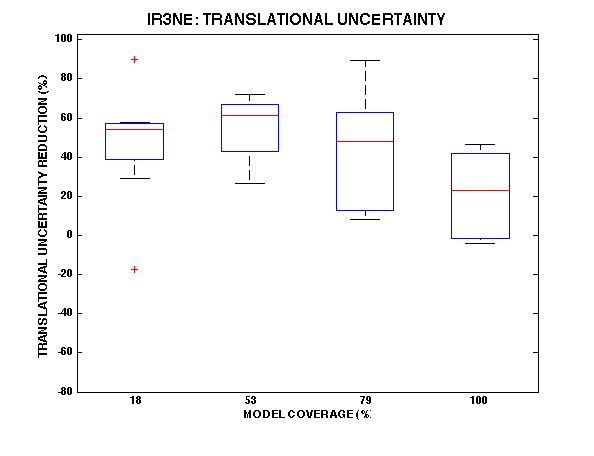
\includegraphics[width=.47\columnwidth]{../media/thesis/img/jug_irene_lin_unc.png}
}
\centerline{
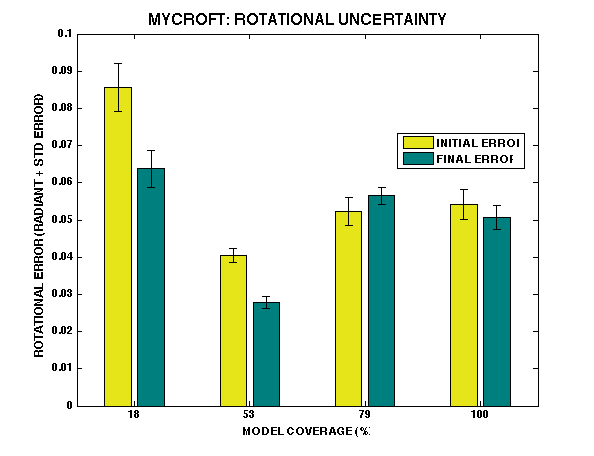
\includegraphics[width=.47\columnwidth]{../media/thesis/img/jug_mycroft_rot_unc.png}
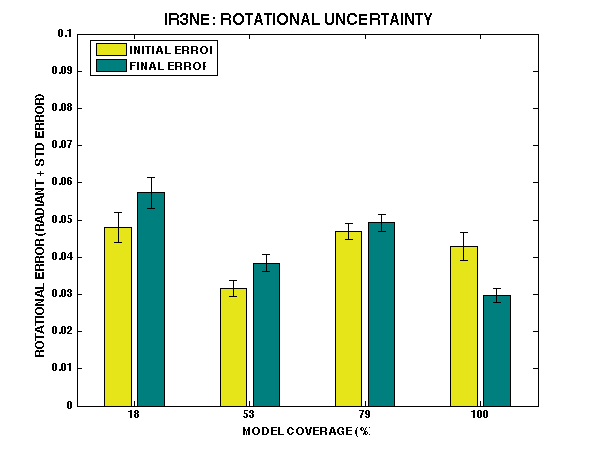
\includegraphics[width=.47\columnwidth]{../media/thesis/img/jug_irene_rot_unc.png}
}

\caption[Simulated results on a jug]{Simulated results for 120 trials on a jug. Three strategies were tested: ELEMENTARY (green), MYCROFT (blue), IR3NE (red). All the results are plotted against the initial percentage of model coverage for a total of four conditions. The top left chart presents the averaged number of iterations across the trials to reach a grasp. The top right chart shows the success rates across the trials. The middle row shows how the initial linear uncertainty (in percentile) is reduced by sequential re-planning until the algorithms converge to a grasp. The bottom row presents the reduction in the rotational uncertainty. Yellow bars represent the initial rotational error, while green bars are the final error. The rotational error is computed in quaternions.}
\label{fig:07:jug_results}
\end{figure}

%Simulated results for 120 trials on a jug. Three strategies: ELEMENTARY (green), MYCROFT (blue), IR3NE (red). All the results are presented plotted against the initial percentage of model coverage given by one or more views by the depth camera. The first chart (top left) presents the average number of iterations required to converge to a grasp. IR3NE shows that maximising information gain requires fewer re-planning iterations to achieve a grasp. The second chart (top right) shows that sequential re-planning is capable of achieving higher success rates than single grasp attempts in presence of uncertainty. The third chart (bottom left) shows how the initial linear uncertainty is reduced by sequential re-planning until the algorithm converges to a grasp. Trajectories that maximise information gain (IR3NE) are capable of localising the objects with a better accuracy. Finally, the last chart (bottom right) presents the reduction in the rotational uncertainty. In this case simple re-planning (MYCROFT) shows better performance, however the rotational uncertainty is usually low for asymmetric objects like the object we used for the experiments.

\begin{figure}[!h]
\centerline{
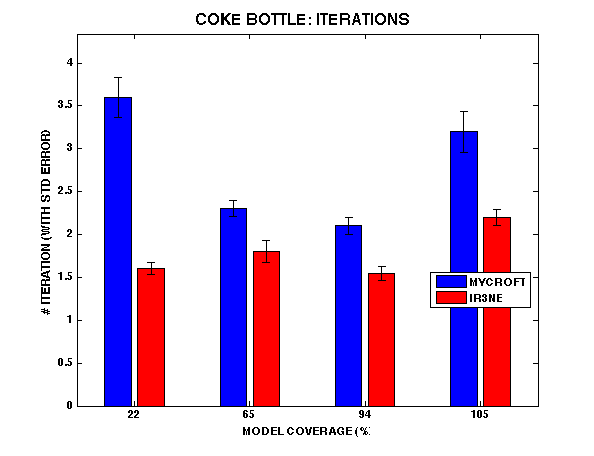
\includegraphics[width=.47\columnwidth]{../media/thesis/img/coke_iterations.png}
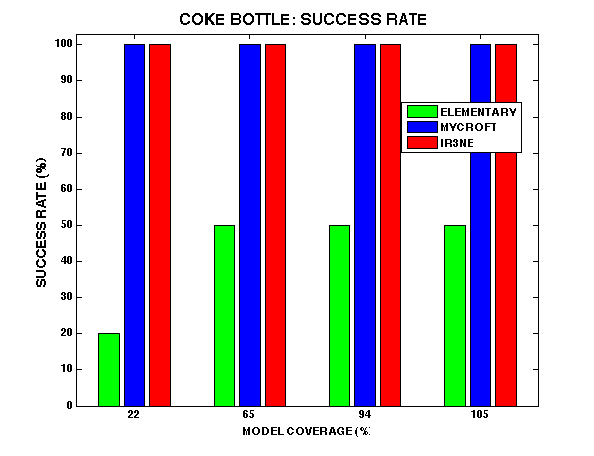
\includegraphics[width=.47\columnwidth]{../media/thesis/img/coke_success_rate.png}
}
\centerline{
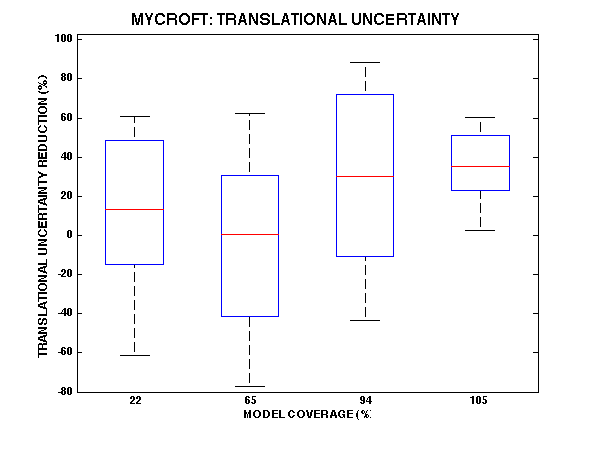
\includegraphics[width=.47\columnwidth]{../media/thesis/img/coke_mycroft_lin_unc.png}
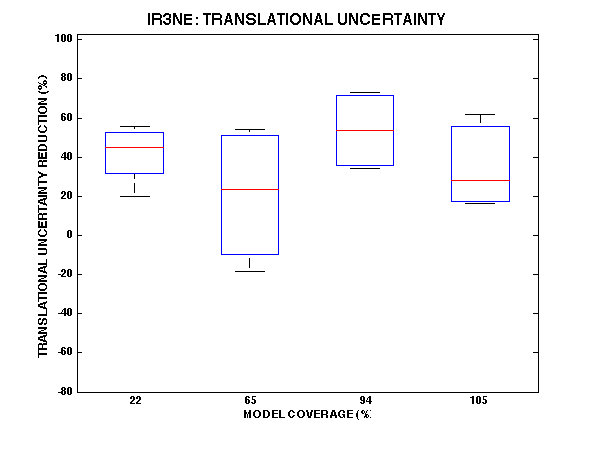
\includegraphics[width=.47\columnwidth]{../media/thesis/img/coke_irene_lin_unc.png}
}
\centerline{
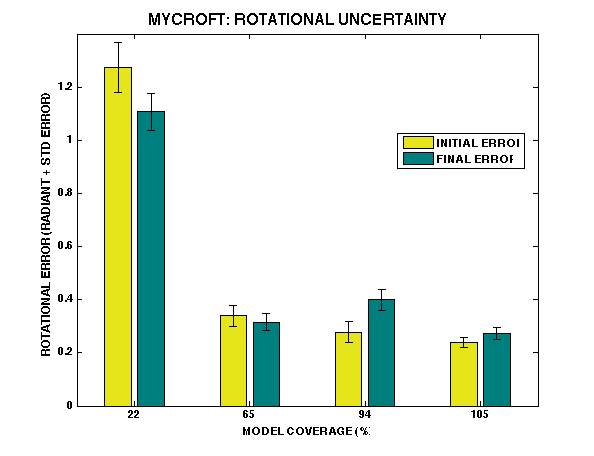
\includegraphics[width=.47\columnwidth]{../media/thesis/img/coke_mycroft_rot_unc.png}
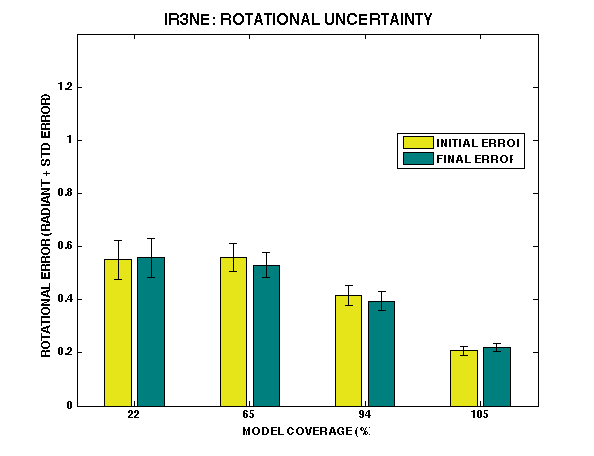
\includegraphics[width=.47\columnwidth]{../media/thesis/img/coke_irene_rot_unc.png}
}

\caption[Simulated results on a coke bottle]{Simulated results for 120 trials on a coke bottle. Three strategies were tested: ELEMENTARY (green), MYCROFT (blue), IR3NE (red). All the results are plotted against the initial percentage of model coverage for a total of four conditions. The top left chart presents the averaged number of iterations across the trials to reach a grasp. The top right chart shows the success rates across the trials. The middle row shows the linear uncertainty reduction (in percentile), while the bottom row presents the reduction in the rotational uncertainty. Yellow bars represent the initial rotational error, while green bars are the final error. The rotational error is computed in quaternions.}
\label{fig:07:coke_results}
\end{figure}

\begin{figure}[!ht]
\centerline{
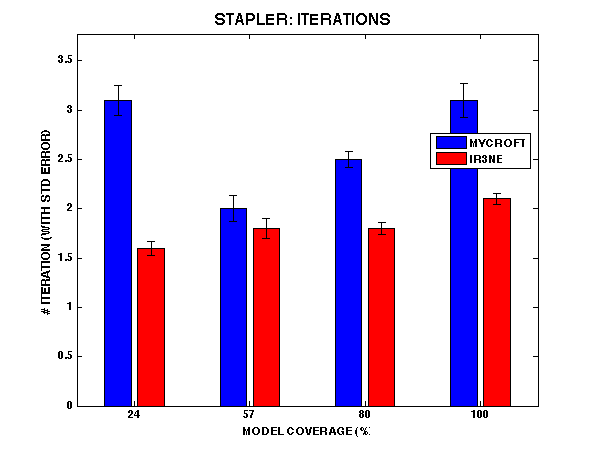
\includegraphics[width=.47\columnwidth]{../media/thesis/img/stapler_iterations.png}
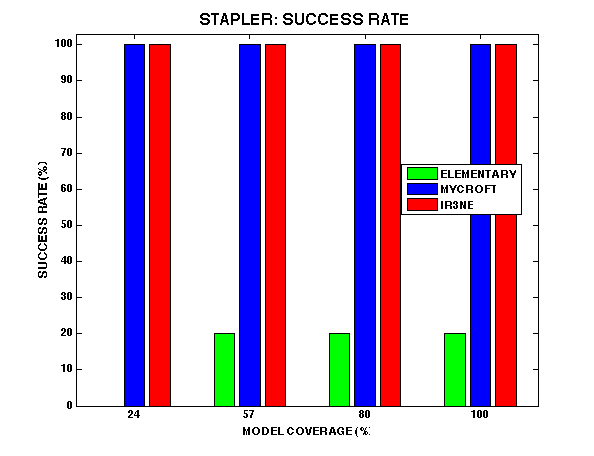
\includegraphics[width=.47\columnwidth]{../media/thesis/img/stapler_success_rate.png}
}
\centerline{
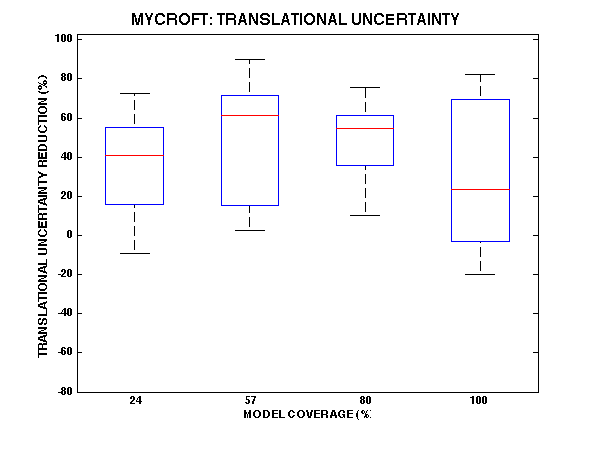
\includegraphics[width=.47\columnwidth]{../media/thesis/img/stapler_mycroft_lin_unc.png}
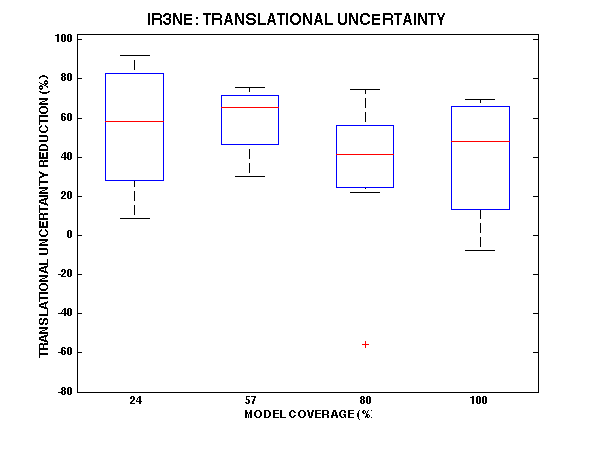
\includegraphics[width=.47\columnwidth]{../media/thesis/img/stapler_irene_lin_unc.png}
}
\centerline{
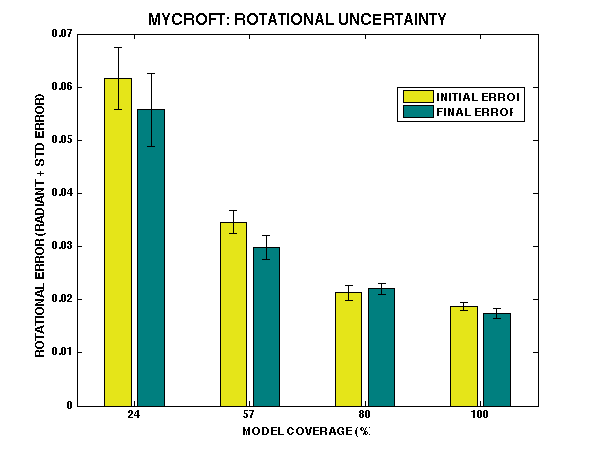
\includegraphics[width=.47\columnwidth]{../media/thesis/img/stapler_mycroft_rot_unc.png}
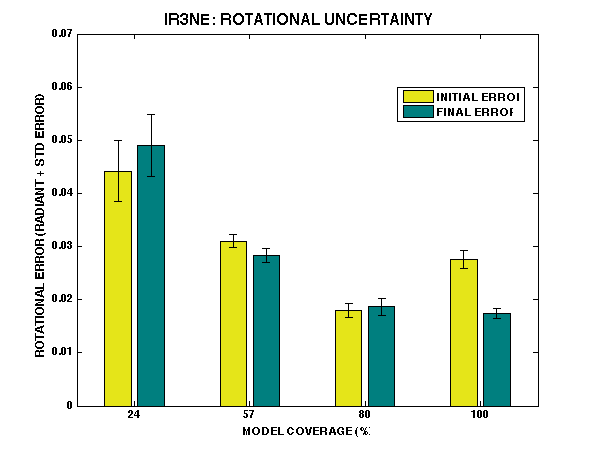
\includegraphics[width=.47\columnwidth]{../media/thesis/img/stapler_irene_rot_unc.png}
}

\caption[Simulated results on a stapler]{Simulated results for 120 trials on a stapler. Three strategies were used: ELEMENTARY (green), MYCROFT (blue), IR3NE (red). All the results are plotted against the initial percentage of model coverage for a total of four conditions. The top left chart presents the averaged number of iterations across the trials to reach a grasp. The top right chart shows the success rates across the trials. The middle row shows the linear uncertainty reduction (in percentile), while the bottom row presents the reduction in the rotational uncertainty. Yellow bars represent the initial rotational error, while green bars are the final error. The rotational error is computed in quaternions.}
\label{fig:07:stapler_results}
\end{figure}

\begin{figure}[!ht]
\centerline{
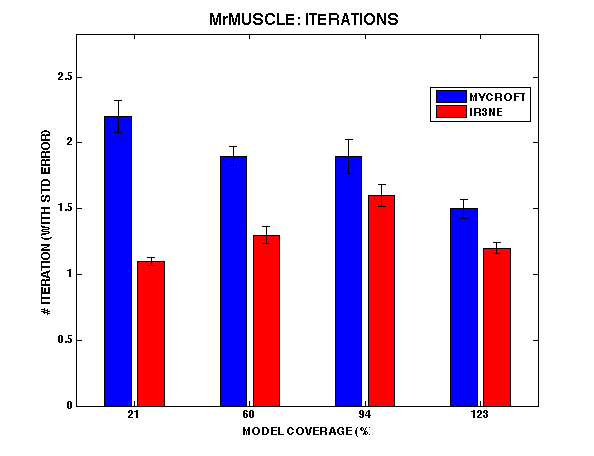
\includegraphics[width=.47\columnwidth]{../media/thesis/img/mrmuscle_iterations.png}
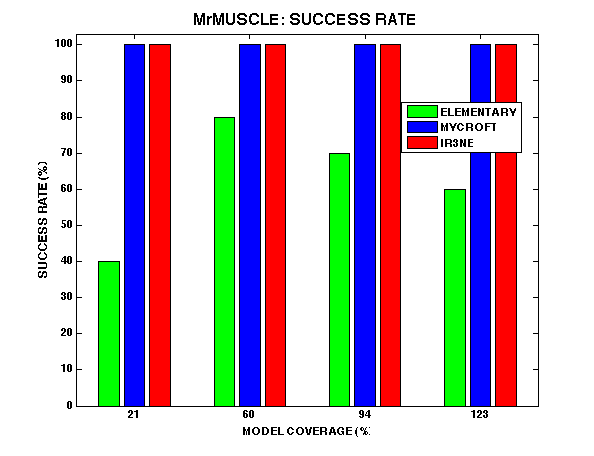
\includegraphics[width=.47\columnwidth]{../media/thesis/img/mrmuscle_success_rate.png}
}
\centerline{
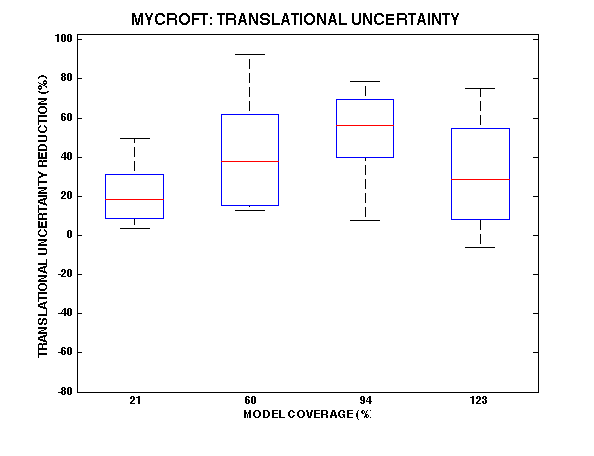
\includegraphics[width=.47\columnwidth]{../media/thesis/img/mrmuscle_mycroft_lin_unc.png}
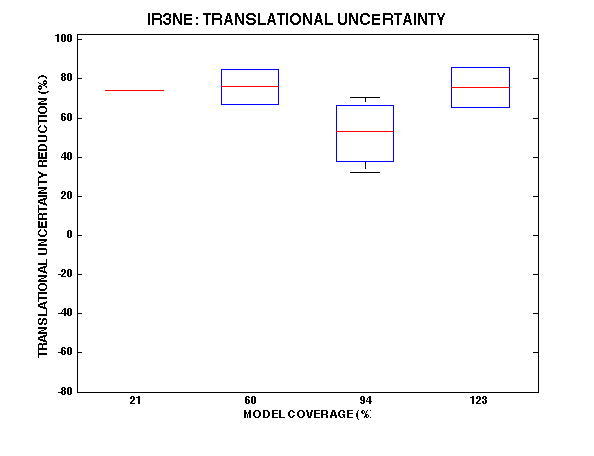
\includegraphics[width=.47\columnwidth]{../media/thesis/img/mrmuscle_irene_lin_unc.png}
}
\centerline{
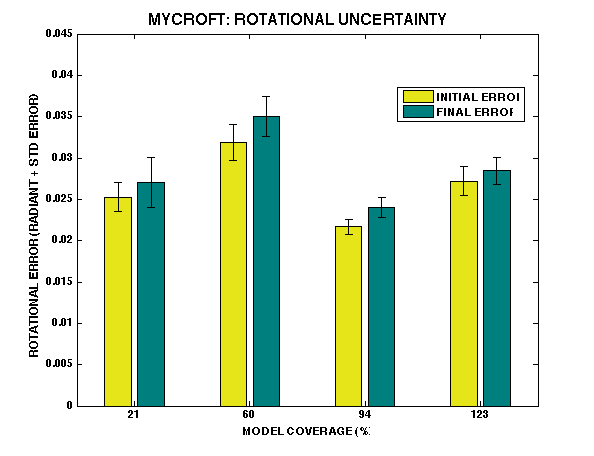
\includegraphics[width=.47\columnwidth]{../media/thesis/img/mrmuscle_mycroft_rot_unc.png}
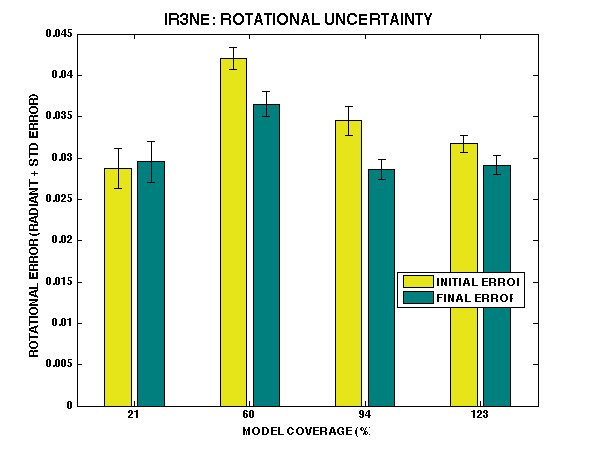
\includegraphics[width=.47\columnwidth]{../media/thesis/img/mrmuscle_irene_rot_unc.png}
}

\caption[Simulated results on a mr muscle spray]{Simulated results for 120 trials on a mr muscle spray. Three strategies were used: ELEMENTARY (green), MYCROFT (blue), IR3NE (red). All the results are plotted against the initial percentage of model coverage for a total of four conditions. The top left chart presents the averaged number of iterations across the trials to reach a grasp. The top right chart shows the success rates across the trials. The middle row shows the linear uncertainty reduction (in percentile), while the bottom row presents the reduction in the rotational uncertainty. Yellow bars represent the initial rotational error, while green bars are the final error. The rotational error is computed in quaternions.}
\label{fig:07:mrmuscle_results}
\end{figure} 

%
%
%---------------------------------------------------------------------------------------------------------------------
% 	CONCLUSION AND FUTURE WORK
%---------------------------------------------------------------------------------------------------------------------
%---------------------------------------------------------------------------------------------------------------------
\newpage
\section{Discussion}\label{sec:ch06_summary}

In this section we discuss the results presented in the previous section.

\subsection{Sequential re-planning in a real scenario}\label{sec:07:boris_discussion}

Figure~\ref{fig:07:jug_boris_results} presents the collected results on the Boris robot platform, as described in Sec.~\ref{sec:07:boris_results}. The results show the benefits of using the hierarchical clustering algorithm to address explicitly the multi-modal nature of the belief space. In particular, the bottom row shows that, in the case of the jug, this approach leads to a lower initial rotational uncertainty with respect to a single mean-shift approach. This is due to the fact that, if the handle of the jug is not visible from the query point cloud, the object looks almost symmetric, which results in a multi-modal rotational uncertainty. Figure~\ref{fig:07:boris.exec.example} shows this case from one of the trials from the collected results. Nevertheless, IR3NE is capable of achieving a grasp in a single iteration, thanks to a more robust approaching trajectory with respect to the estimated uncertainty. 

These two sets of trials have shown the validity of the sequential re-planning approach on a real scenario, however there are several issues that have to be addressed. First, the need for a predictive model for predicting how the target object moves after a contact occurs. Although the contact detection module described in Sec.~\ref{sec:07:detecting_contacts} reliably stops the robot after a contact is made, light objects, such as the plastic jug used in these trials, may be perturbed by the contact. For example, often we observe that the jug is tilted by a finger. The belief update by itself cannot deal with these cases and the resulting mean estimations are usually incorrect. However, the choice of point cloud models negatively affects the ability of developing predictive models.
Second, the lack of tactile sensors does not allow us to have a good estimate of which link of the finger experienced the contact. This results in an additional uncertainty in the belief update. 

\begin{figure}[!t]
  \centering
  \begin{subfigure}[t]{0.28\textwidth}
       \includegraphics[width=4.cm]{../media/thesis/img/boris_00_query.png}
       \caption{}\label{fig:07:boris_irene_01}
  \end{subfigure} 
  \quad
  \begin{subfigure}[t]{0.28\textwidth}
     \includegraphics[width=4cm]{../media/thesis/img/boris_00_belief.png}
     \caption{}\label{fig:07:boris_irene_02}
  \end{subfigure}
  \quad
  \begin{subfigure}[t]{0.28\textwidth}
     \includegraphics[width=4cm]{../media/thesis/img/boris_01.png}
     \caption{}\label{fig:07:boris_irene_03}
  \end{subfigure}
\vspace{2mm}

 \begin{subfigure}[t]{0.28\textwidth}
       \includegraphics[width=4cm]{../media/thesis/img/boris_03.png}
       \caption{}\label{fig:07:rboris_irene_04}
  \end{subfigure} 
  \quad
  \begin{subfigure}[t]{0.28\textwidth}
     \includegraphics[width=4cm]{../media/thesis/img/boris_04.png}
     \caption{}\label{fig:07:rboris_irene_05}
  \end{subfigure}
  \quad
  \begin{subfigure}[t]{0.28\textwidth}
     \includegraphics[width=4cm]{../media/thesis/img/boris_05.png}
     \caption{}\label{fig:07:boris_irene_06}
  \end{subfigure}
\vspace{2mm}

 \begin{subfigure}[t]{0.28\textwidth}
       \includegraphics[width=4cm]{../media/thesis/img/boris_07.png}
       \caption{}\label{fig:07:boris_irene_07}
  \end{subfigure} 
  \quad
  \begin{subfigure}[t]{0.28\textwidth}
     \includegraphics[width=4cm]{../media/thesis/img/boris_08.png}
     \caption{}\label{fig:07:boris_irene_08}
  \end{subfigure}
  \quad
  \begin{subfigure}[t]{0.28\textwidth}
     \includegraphics[width=4cm]{../media/thesis/img/boris_10.png}
     \caption{}\label{fig:07:boris_irene_10}
  \end{subfigure}
\vspace{2mm}

 \caption[SPAM-PLAN results on Boris]{Example of plan execution for IR3NE. The top row shows:~\subref{fig:07:boris_irene_01} the partial query point cloud (3 merged views),~\subref{fig:07:boris_irene_02} the belief state (as sub-sampled hypotheses (blue), mean pose (green) and ground truth (black)),~\subref{fig:07:boris_irene_03} the real pose of the object. This example shows the worst case in which the the query point cloud covers only a 22.5\% of the model and the handle is not visible. Note that the ground truth~\subref{fig:07:boris_irene_02} (black point cloud) is also estimated with the wrong orientation. Nevertheless, IR3NE executes the planned trajectory (middle row) and achieve e grasp~\subref{fig:07:boris_irene_07} and~\subref{fig:07:boris_irene_08}. In~\subref{fig:07:boris_irene_10}, Boris lifts successfully the jug.}
\label{fig:07:boris.exec.example}
\end{figure} 

Future work aims to address such issues by extending the sequential re-planning approaches to the use of tactile sensors and simple heuristics for an object-independent predictive model. The latter should be based on simple geometric properties of non-penetration between objects and robot's fingers to constrain the belief update and the mean pose estimate.   


\subsection{Sequential re-planning in a virtual scenario}\label{sec:07:simulated_results_discussion}

\begin{figure}[!ht]
  \centering
  \begin{subfigure}[t]{0.4\textwidth}
       \includegraphics[height=3.9cm,width=5.4cm]{../media/thesis/img/query.png}
       \caption{}\label{fig:07:replan_1}
  \end{subfigure} 
  \quad
  \begin{subfigure}[t]{0.4\textwidth}
     \includegraphics[height=3.9cm,width=5.4cm]{../media/thesis/img/trial_01.png}
     \caption{}\label{fig:07:replan_2}
  \end{subfigure}
 \quad
  \begin{subfigure}[t]{0.4\textwidth}
       \includegraphics[height=3.9cm,width=5.4cm]{../media/thesis/img/trial_02.png}
       \caption{}\label{fig:07:replan_3}
  \end{subfigure} 
 \vspace{2mm}
  \begin{subfigure}[t]{0.4\textwidth}
     \includegraphics[height=3.9cm,width=5.4cm]{../media/thesis/img/trial_03.png}
     \caption{}\label{fig:07:replan_4}
  \end{subfigure}
   \quad
  \begin{subfigure}[t]{0.4\textwidth}
       \includegraphics[height=3.9cm,width=5.4cm]{../media/thesis/img/trial_04.png}
       \caption{}\label{fig:07:replan_5}
  \end{subfigure} 
%  \centerline{
%\includegraphics[height=5.0cm,width=.48\columnwidth]{../media/thesis/img/trial_01.png}
%\includegraphics[height=5.0cm,width=.48\columnwidth]{../media/thesis/img/trial_02.png}
%}
%\vspace{.8}
%\centerline{
%\includegraphics[height=5.0cm,width=.48\columnwidth]{../media/thesis/img/trial_03.png}
%\includegraphics[height=5.0cm,width=.48\columnwidth]{../media/thesis/img/trial_04.png}
%}
\caption[SPAM-PLAN simulated results]{Example of plan execution for IR3NE. Top row: a partial point cloud is acquired~\subref{fig:07:replan_1} and a density distribution represented by a set of particles is computed and a reach-to-grasp trajectory is planned~\subref{fig:07:replan_2}. The red point cloud identifies the ground truth which exactly matches the partial point cloud in~\subref{fig:07:replan_1}. The blue point clouds represent the low dimensional belief states sub-sampled from the corresponding high dimensional belief states. The yellow point cloud represents the estimated pose for the object. Second row: despite the tiny misplacement between the estimate pose and the ground truth, a contact occurs before the grasp configuration with respect to the mean pose (yellow point cloud) could be reached~\subref{fig:07:replan_3}. The belief state is therefore updated from the contact~\subref{fig:07:replan_4} and a new trajectory is planned with respect to the new estimate. Bottom row: the hand reaches the target grasp pose~\subref{fig:07:replan_4}.}
\label{fig:07:spam.exec.example}
\end{figure}  

The results collected in the virtual scenario confirms the ability of the sequential re-planning approach to achieve a grasp more robustly than a single grasp attempt (ELEMENTARY strategy) for all the objects (Fig~\ref{fig:07:grasps}) and all the conditions (see Sec~\ref{sec:07:simulated_results}). In addition, Sec~\ref{sec:07:simulated_results} has also shown that IR3NE is capable of achieving successful grasps with fewer iterations than MYCROFT.

To illustrate the behaviour of the re-planning system Fig.~\ref{fig:07:spam.exec.example} shows a typical sequence generated by one simulation trial attempting to perform a rim grasp on the jug. In this case the initial belief state over the object pose is quite narrow (Fig.~\ref{fig:07:replan_2}), however an error of a few millimetres in the pose estimate leads to a potentially dangerous contact with the object (Fig.~\ref{fig:07:replan_3}). The contact is used to update the belief and plan a new trajectory from the current configuration of the robot(Fig.~\ref{fig:07:replan_4}). The second trajectory successfully transfers the hand to the target grasp configuration (Fig.~\ref{fig:07:replan_5}).



\section{Conclusion}\label{sec:ch07:summary}

This chapter has shown the validity, via empirical results, of the sequential re-planning algorithms on a real scenario. In addition, this approach has been evaluated in a simulated environment on four different objects. Several innovations have been developed to extend the theoretical techniques of Chap.~\ref{ch06}, to overcome difficult practical problems encountered when trying to implement simultaneous perception and grasping with a real robot manipulator with 21 DoF and non-Gaussian object pose uncertainty in 6D, as well as incomplete knowledge of the object shape.

The main contribution of this chapter is to describe, demonstrate and evaluate a novel approach for the problem of robot grasping, where a robot is capable of reasoning about object-pose uncertainty while planning a dexterous reach-to-grasp trajectory. This system shown in Fig~\ref{fig:architecture} is able to plan grasp operations autonomously in unstructured environments, with no knowledge of the object we wish to manipulate, apart from a model point cloud. 

As in Chap~\ref{ch06},  this chapter has shown how sequential re-planning can achieve better quality grasps than single attempts to directly grasp an object at its expected pose, and that re-planning with trajectories designed to maximise tactile information gain, achieves successful grasps with fewer iterations than sequential attempts to move directly towards the object's expected pose.


